\chapter{Introduction}

In satellite applications, radio communication is the most important method for controlling the satellite state and issuing any commands to it. 

\section{Aim of the thesis}

The aim of this thesis was to design, test \& deploy communication system for second Polish satellite, PW-Sat2. This work covers phases of component selection \& design, testing all the subsystems and finally results from the on-orbit mission.

\section{PW-Sat2}
    The presented system was design specifically to be deployed on-board the PW-Sat2 satellite \cite{PW-Sat2URL}. PW-Sat2 was launched on Low Earth Orbit or 3rd of December 2018 on-board Falon9 rocket from SpaceX company.

    In the figure \ref{PW-Sat_render_01} an exploded render of PW-Sat2 is presented.
    
    %%% [TODO]: JAKIEŚ ZDJĘCIA

    \begin{figure}[H]
        \centering
        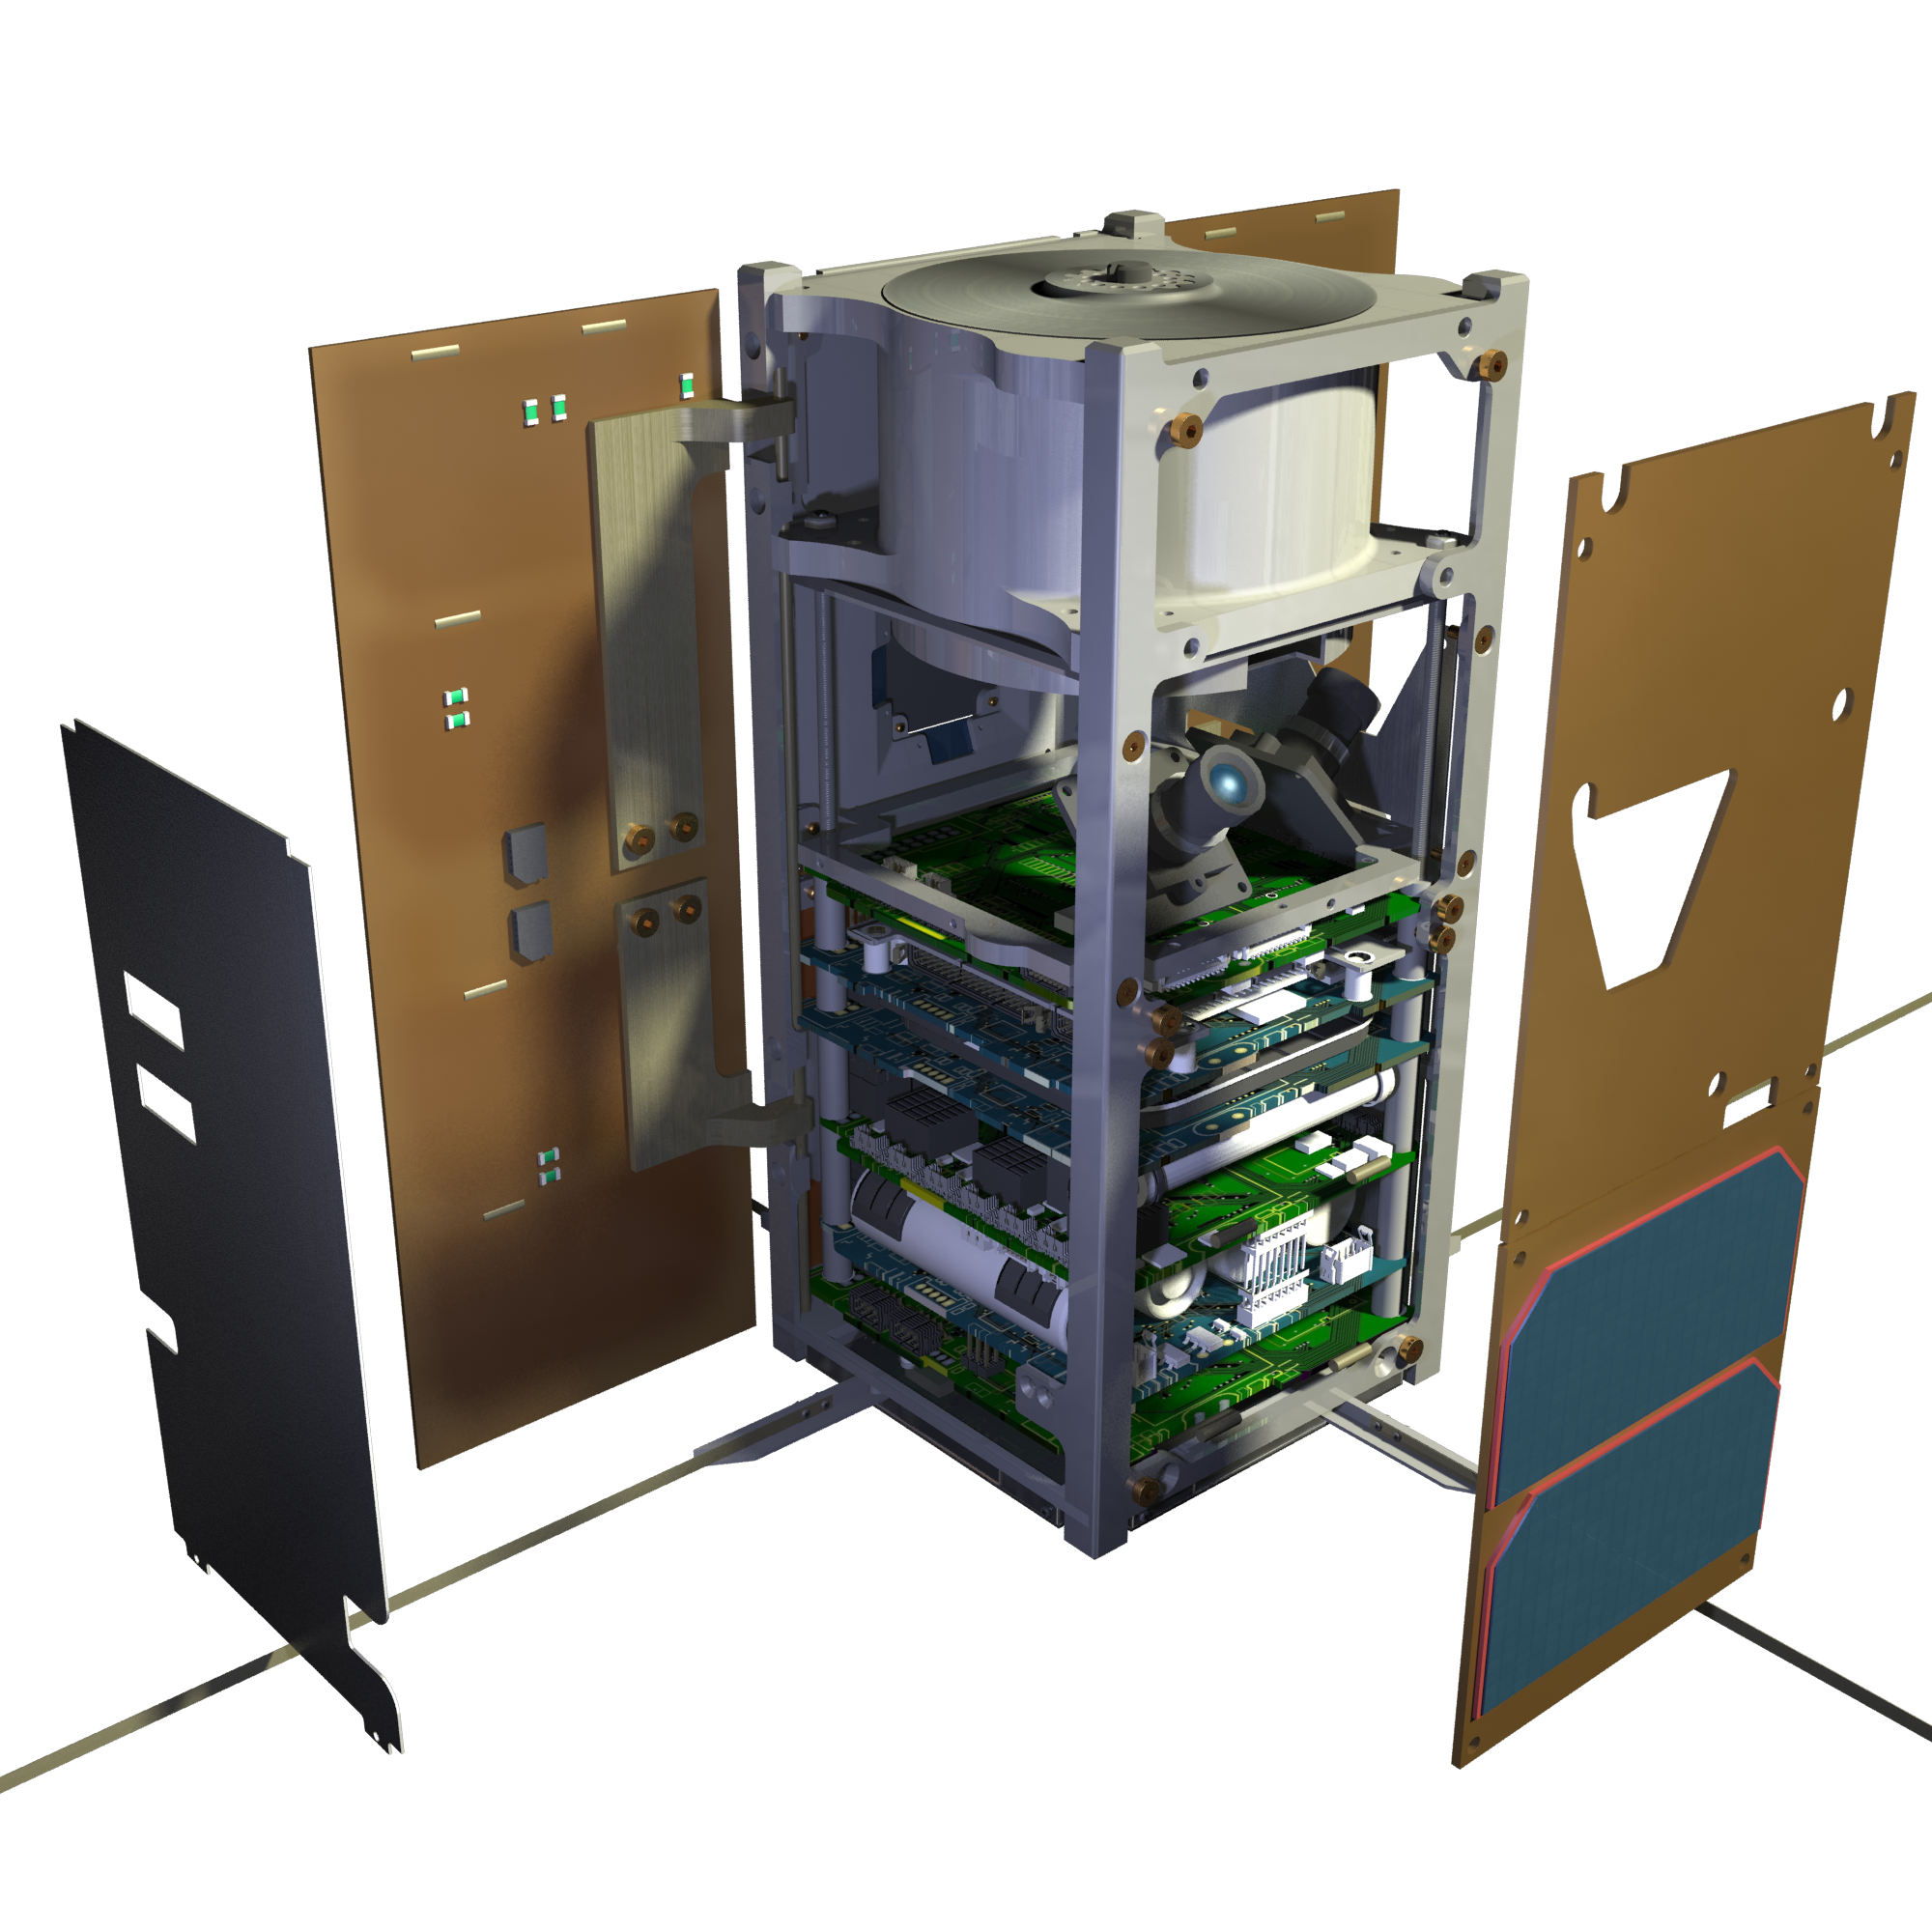
\includegraphics[width=0.65\paperwidth]{img/4/PW-Sat2_render_01.png}
        \caption{PW-Sat2 render. Source: \cite{PW_sat2_photo}}
        \label{PW-Sat_render_01}
    \end{figure}


    \subsection{Primary mission}
    % skopiowane z inż, do przepisania
        The primary mission of PW-Sat2 is to test the deorbit sail. When satellite mission ends, it has to be safely deorbited (or moved to graveyard orbit). Due to new regulations, satellite has to be removed from
        the LEO region no later than 25 years after the end of vehicle operations \cite{Satellite_disposal}. Purpose of deorbit sail is, after satellite operations, to open and increase atmospheric drag, shortening satellite life and cause deorbitation. More information about this experiment can be found in \cite{DDC_article}.

        A render of PW-Sat2 with opened sail is shown in the figure \ref{PW-Sat_render_sail}.

        \begin{figure}[H]
            \centering
            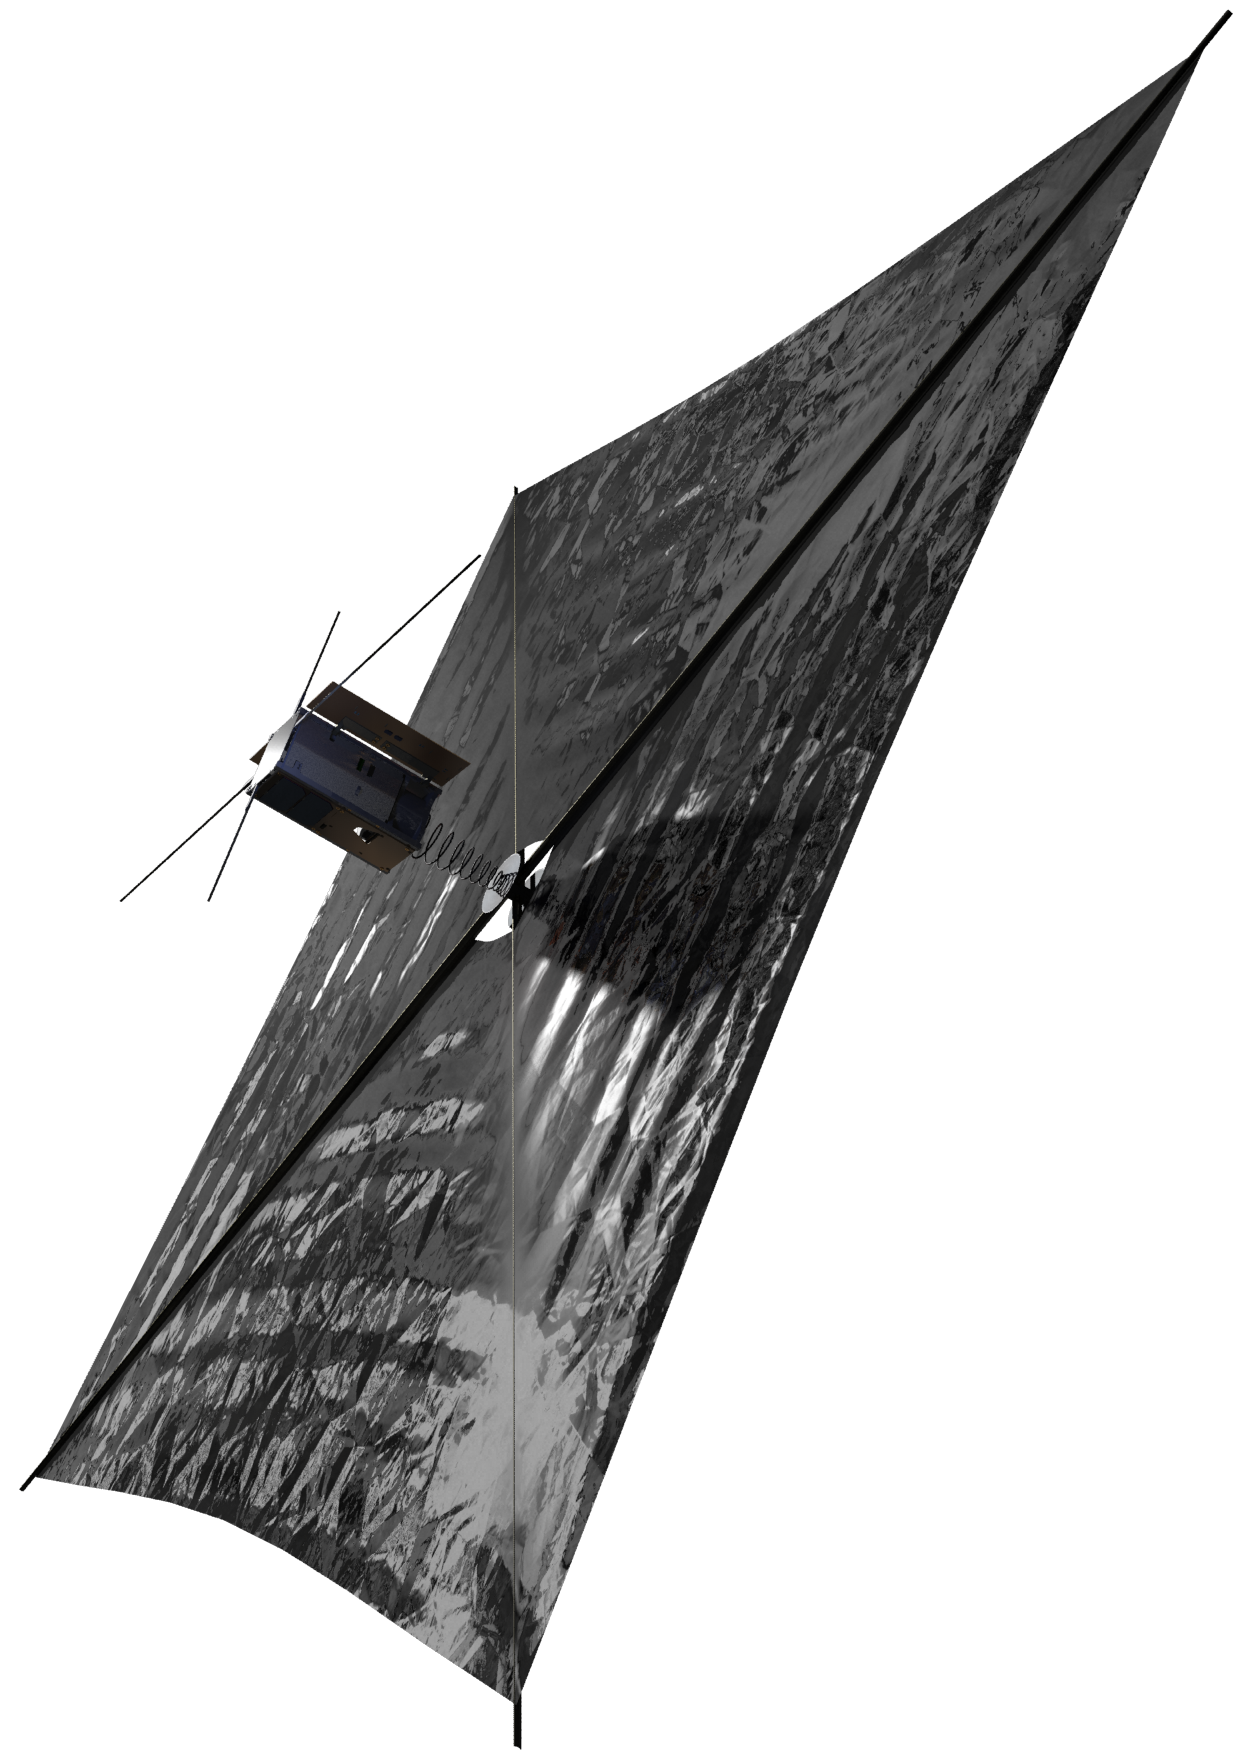
\includegraphics[width=0.38\paperwidth]{img/4/PW-Sat2_render_02.png}
            \caption{PW-Sat2 with opened sail. Source: \cite{PW_sat2_photo}}
            \label{PW-Sat_render_sail}
        \end{figure}

    \subsection{Mission plan and system lifetime}
        PW-Sat2 mission was divided into two phases: normal \& extended mission. Normal phase was planned to take 40 days, after which the deorbitation phase and extended mission begin. Deorbitation can  take up two two years, during which its state along with satellite housekeeping should be monitored.

    \subsection{Orbit}
        PW-Sat2 in planned to be launched to a sun-synchronous circular orbit of attitude \SI{575}{\kilo\meter}, with LTAN of 10:30 \cite{PWSAT_MA_CDR}.



\section{Low Earth Orbit satellite communication review}



\section{Requirements for the system}